\documentclass[10pt]{article}
\usepackage[margin=1.13cm]{geometry}
\usepackage{array, xcolor}
\usepackage{lipsum}
\usepackage{setspace}
\usepackage{enumitem}
\usepackage{hyperref}
\usepackage{graphics}
\usepackage {graphicx}
\usepackage{mathpazo}   % Uses Palatino fonts - Much much better then usual Computer Modern, suggested by Prof. VPS.
%\usepackage{palatino}
\title{\bfseries\LARGE Maulik C. Madhavi}
\author{\normalsize Research Fellow, Department of Electrical and Computer Engineering, NUS, Singapore\\%Ph.D. (DA-IICT), M.Tech (DA-IICT), B.E. (E.C.)
\normalsize Email: maulik.madhavi@nus.edu.sg, maulikmadhavi@gmail.com, (Ph): +65-85443713}
%\normalsize Personal website: \href{https://sites.google.com/site/maulikcmadhavi}{https://sites.google.com/site/maulikcmadhavi}\\{\normalsize Github: \href{https://github.com/maulikmadhavi/}{https://github.com/maulikmadhavi/}}}}
\date{}
\begin{document}
\maketitle


\definecolor{lightgray}{gray}{0.8}
\newcolumntype{L}{>{\raggedleft}p{0.19\textwidth}}
\newcolumntype{R}{p{0.8\textwidth}}
\newcommand\VRule{\color{gray!80}\vrule width 1.5pt}
\setstretch{1.15}          % Sets Line space for the rest of the Thesis. Do not change.                       
%\section*{Goal}
%To understand the complex human speech production mechanism and build real-time, easy accessible, applications for speaking or hearing impaired people as well as for common man.

\section*{Research and Technical Experience}
\begin{tabular}{L!{\VRule}R}
	Dec, 2017-Present&\textbf{Designation}: Research Fellow \\
	& \href{http://ece.nus.edu.sg/hlt/maulik/}{National University of Singapore (NUS)}\\
	%	&\textbf{Title}: Neuromorphic Computing\\
	&\textbf{Project activities}:  Chatbot for autonomous vehicle, Text-dependent speaker verification, ASR for healthcare calls, Form filling system.\\
	&\textbf{PI}: Prof. Haizhou Li \vspace{0.3cm}\\
	&\textbf{Others}: Mentor and co-supervise the final year undergrad students for \href{https://drive.google.com/drive/folders/1XS0ttBsnD0YT5Y_pZ_QEw_XN3gmKMIOT}{their projects}.
	
	\\
	%\vspace{0.4cm}\\
	April, 2012-June, 2014&\textbf{Designation}: Project Personnel, \href{https://sites.google.com/site/speechlabdaiict/projects/prosodically-guided-phonetic-engine-development}{DA-IICT, Gandhinagar} \\
	&\textbf{Project activities}: Prosodically Guided Phonetic Engine Development
	for Gujarati and Marathi languages \\
	& Dhirubhai Ambani Institute of Information and Communication Technology (DA-IICT)\\
	&\textbf{PI}: Prof. Hemant Patil\\
	%&\textbf{Funding Agency}: Department of Electronics and Information Technology (DeitY), 	Govt. of India.\\
	
	%&\textbf{Duties}: \vspace{0.1cm}
	%\begin{itemize}
	%		\setlength\itemsep{0em}
	%	\item To collect speech data in Gujarati and Marathi languages. 
	%	\item To Guide and monitor consultants for the manual phonetic transcription and syllabification task.  
	%	\item 	Develop phonetic engine and search engine for Gujarati and Marathi languages. 
	
\end{tabular}


%\begin{figure}[h]
%	\centering
%\href{http://ece.nus.edu.sg/hlt/st-kinetics-autonomous-bus-trial-2/}{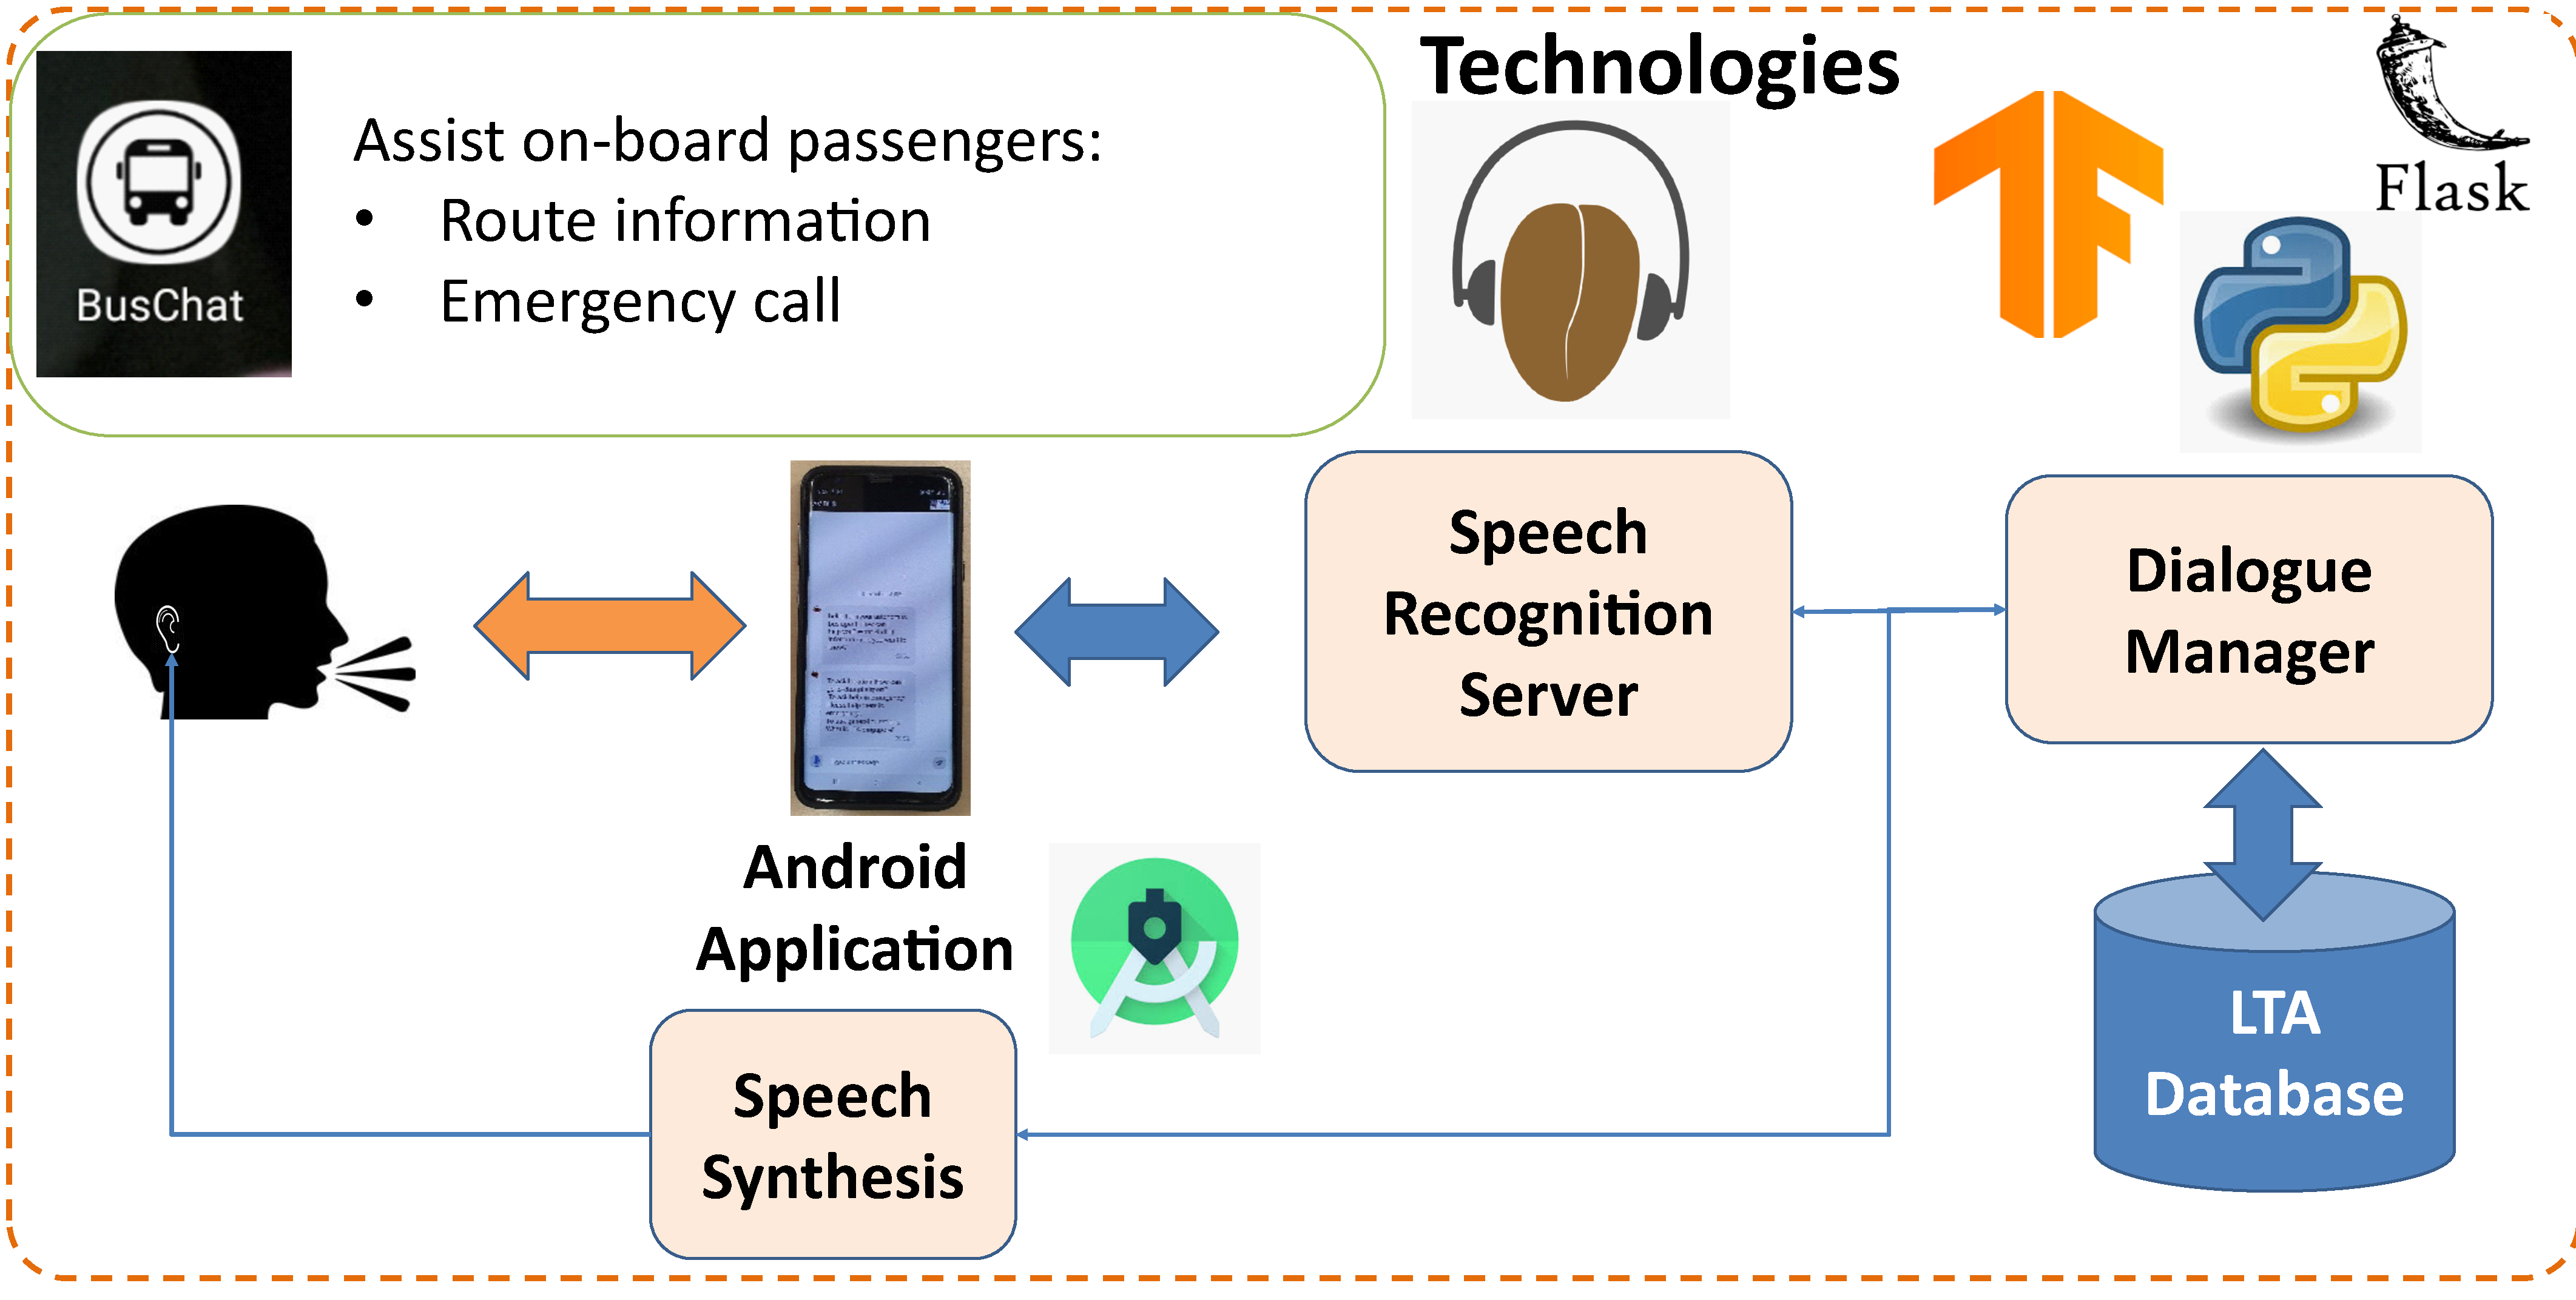
\includegraphics[trim=0 0 0 0, clip,scale=0.15]{Buschat.pdf}}
%\caption{Chatbot for autonomous vehicle}
%\end{figure}
%
%\begin{figure}[h]
%	\centering
%	\href{https://github.com/maulikmadhavi/Hellobus_tflite}{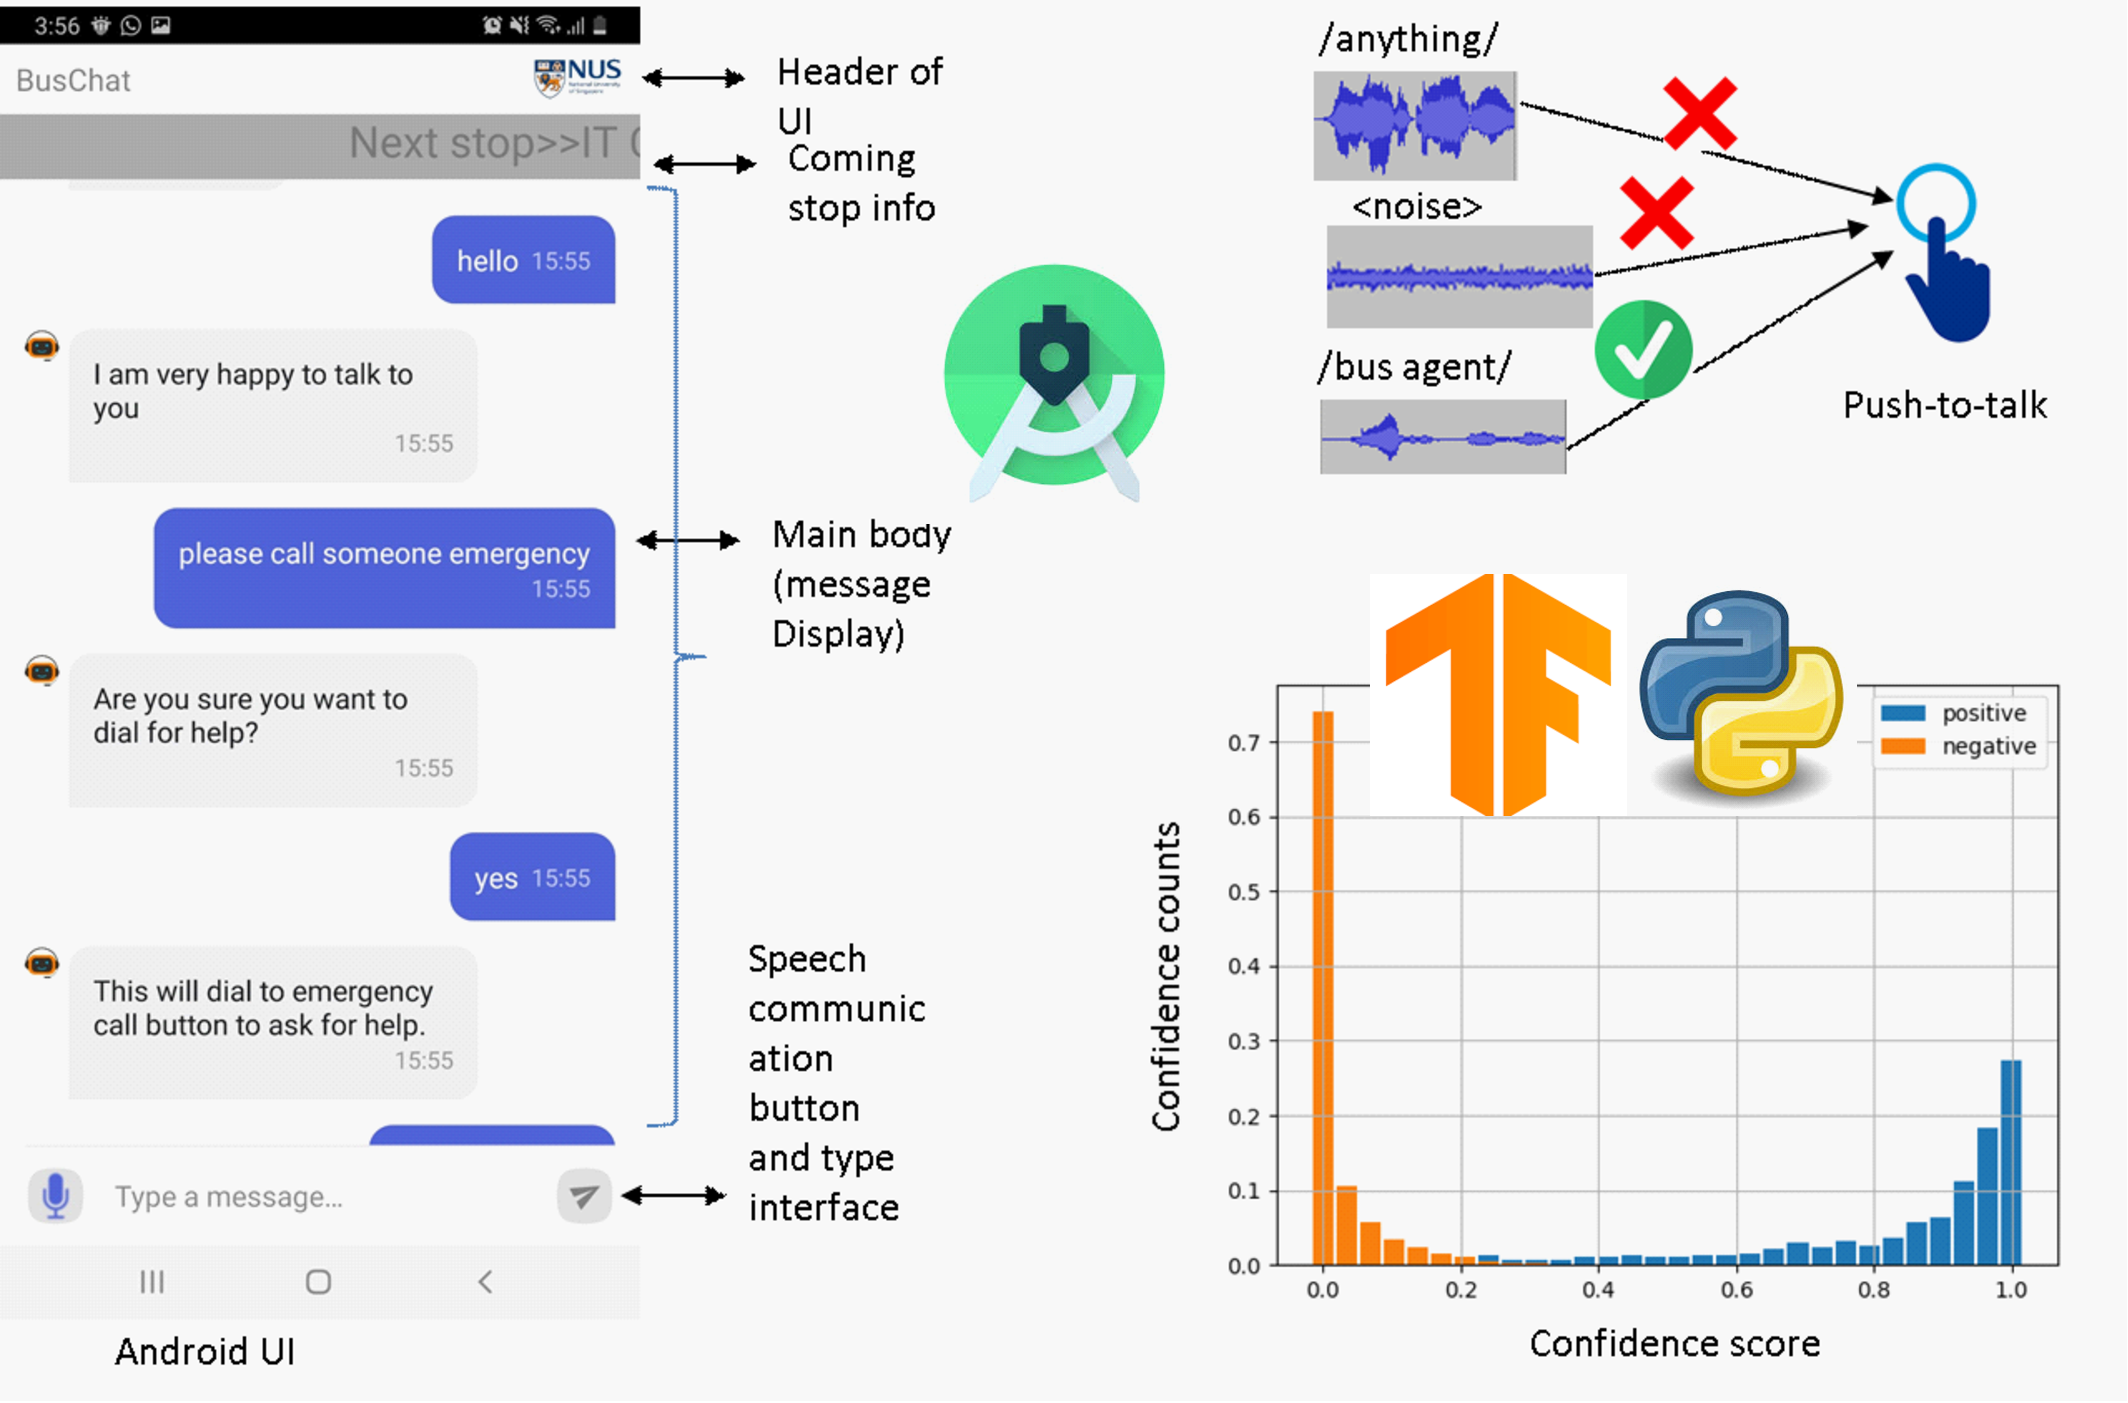
\includegraphics[trim=10 0 0 0, clip,scale=0.2]{wakeupword.pdf}}
%	\caption{Wakeup word ASR (integration to chatbot)}
%\end{figure}


\section*{Education}
\begin{tabular}{L!{\VRule}R}
2011-2017& \textbf{Ph.D., Information and Communication Technology (ICT)}\\& Dhirubhai Ambani Institute of Information and Communication Technology (DA-IICT), Gandhinagar.\\&- CPI 9.75/10 \vspace{0.4cm}\\
2009-2011&\textbf{M.Tech Information Communication Technology (ICT)}, Communication Systems specialization. \\&Dhirubhai Ambani Institute of Information and Communication Technology (DA-IICT), Gandhinagar.\\&- CPI 8.26/10\vspace{0.4cm}\\
2005-2009&\textbf{B.E. Electronics and Communication (EC)}\\&V. V. P. Engg. College, Rajkot (Saurashtra University)\\& Percentage (69.73\%)(aggregate)\vspace{0.3cm}\\
2004-2005&\textbf{H.S.C}\\&Gujarat Secondary and Higher Secondary Education Board\\&- Percentage 85.80 \% (aggregate), 70.77 \%\vspace{0.4cm}\\
2002-2003&\textbf{S.S.C.}\\&Gujarat Secondary and Higher Secondary Education Board\\&- Percentage 82.14\% 
\end{tabular}
\vspace{0.25cm}

\section*{Skills}
\begin{tabular}{L!{\VRule}R}
	Research area: &Speech signal processing, voice search, speaker verification, spoken language understanding, deep learning for spoken language processing.\vspace{0.2cm}\\
	%Programming Lang.:& Unix Shell Scripting, and C/C++\vspace{0.1cm}\\
	Tools:& Bash, C/C++, Android (basic), Python, MATLAB,  Git, Docker, kaldi, Deep learning frameworks (TensorFlow, PyTorch) \vspace{0.2cm}\\
	%Graphic Editor: &Inkscape \vspace{0.1cm}\\
	OS: & Windows and Linux \vspace{0.2cm}\\
	%Documentation: & \LaTeX, Word, HTML, GitHub \vspace{0.1cm}\\
	Google Scholar: & {Citation}: 158, {h-index}: \textbf{7}, {i10-index} : 6 %\vspace{0.2cm}\\
	%Research Gate (RG) score: & \textbf{10.25}
\end{tabular}
% All the consortium meetings were held at IIIT-Hyderabad. Most of the team members of DA-IICT team including principal investigator have attended all the meetings. Details of Project meeting held at IIIT-Hyderabad are shown in Table ~\ref{Training}. 

%\begin{table}[!h]
%	\caption {Attended Deity sponsored consortium project review meetings}
%	%  \begin{small}
%	\centering
%	\begin{tabular}{|p{.5cm}|p{2.5 cm}|p{2.5 cm}|p{5 cm}|p{7cm}|} 
%		\hline \textbf{Sr. No} 		&\textbf{Date of project meeting} 	&\textbf{Organizer}	&\textbf{Participants} 		&\textbf{Agenda}\\		\hline 
%		\hline 
%%		1 &WISP 2011 and Project meeting (Dec, 2011) & Project PI (Prof. Hemant A. Patil) &Project information  \\ \hline
%		1 &18-20 Feb. 2012 & IIIT Hyderabad & Prof. Hemant A. Patil, Maulik C. Madhavi, Kewal D. Malde &Use of phonetic transcription in phonetic engine, Concept of phonetic engine \\ \hline
%		2 &11-13 May 2012 & IIIT Hyderabad &Prof. Hemant A. Patil, Maulik C. Madhavi, Kewal D. Malde, Bhavik B. Vachhani &Phonetic transcription in detail \\ \hline 
%		3 &25-28 October 2012 & IIIT Hyderabad&Prof. Hemant A. Patil, Maulik C. Madhavi, Kewal D. Malde &Signal level information extraction. Syllabification, pitch marking and break marking.   \\ \hline 
%		4 &9-10 March 2013 & Thapar University, Patiala&Prof. Hemant A. Patil, Maulik C. Madhavi, Kewal D. Malde, Bhavik B. Vachhani, Tarunima Prabhakar, Mansi Gokhale & Speech segmentation, common phoneset and benchmarking data preparation, different techniques for search engine.   \\ \hline 
%		5 &12-13 Oct. 2013& DA-IICT, Gandhinagar &Prof. Hemant A. Patil, Maulik C. Madhavi, Ankur Undhad, Shubham Sharma &Audio search, demos of phonetic engine, discussion on prosodic marks (pitch and break mark).\\ \hline 
%		6 &8-9 March 2014 & IIT Kharagpur &  Prof. Hemant A. Patil, Maulik C. Madhavi & Preparation of the phonetic engine systems and discussion on the format of deliverables\\ \hline 
%	\end{tabular}
%	\label{Training}
%\end{table} 

%\newpage
\vspace{0.25cm}
\section*{Research Publications}
\subsubsection*{International Journals}
\begin{enumerate}
				\setlength\itemsep{-0.05em}
\item \textbf{M. C. Madhavi}, and H. A. Patil, ``Vocal Tract Length Normalization using a Gaussian mixture model framework for query-by-example spoken term detection,'' in \textit{Computer, Speech and Language, Elsevier}, vol. 58, pp. 175-202, November 2019.
\item \textbf{M. C. Madhavi}, and H. A. Patil, ``Design of mixture of GMMs for query-by-example spoken term detection,'' in \textit{Computer, Speech and Language, Elsevier}, vol. 52, pp. 41-55, November 2018.
\item H. A. Patil, and \textbf{M. C. Madhavi}, ''Combining evidences from magnitude and phase information using VTEO for person recognition using humming,'' on \textit{special issue of recent advances in speaker and language recognition and characterization Computer Speech and Language, Elsevier}, vol. 52, pp. 225-256, November 2018.
 \item \textbf{M. C. Madhavi}, and H. A. Patil, ''Partial matching and search space reduction for QbE-STD,'' in \textit{Computer Speech \& Language, Elsevier}, vol. 45, pp. 58-82, September 2017.
\item H. A. Patil, \textbf{M. C. Madhavi}, K. K. Parhi, ''Static and dynamic information derived from source and system features for person recognition from humming,'' \textit{Int. Journal of Speech Technology, Springer} , vol. 15, no. 3, pp. 393-406, 2012. 
\end{enumerate}
\subsubsection*{Book Chapters}
\begin{enumerate}[resume]
				\setlength\itemsep{-0.05em}
	\item \textbf{M. C. Madhavi}, H. A. Patil and N. Bhendawade, ``Spoken Keyword Retrieval using Source and System Features,''  Pattern Recognition and Machine Intelligence. PReMI 2017,  B. Uma Shankar et. al. (Eds), Lecture Notes in Computer Science (LNCS), pp. 333-341, 2017. 
%	\item \textbf{M. C. Madhavi}, and H. A. Patil, ``A method to alleviate performance degradation in template matching for query in isolation,'' Int. Conf. on Speech and Computer (SPECOM), Hatfield, Hertfordshire, UK, Sep 12-16, 2017. 
	\item 	\textbf{M. C. Madhavi}, S. Sharma, H. A. Patil, ``VTLN Using different warping functions for template matching,'' \textit{Machine Intelligence and Big Data in Industry}, Springer International Publishing,  D. Ry{\.{z}}ko, P. Gawrysiak, M. Kryszkiewicz, and H. Rybi{\'{n}}ski, Henryk (Eds.),  pp. 111-121, 2016. 
	\item \textbf{M. C. Madhavi}, S. Sharma, and H. A. Patil, ``Vocal tract length normalization features for audio search,'' in \textit{Int. Conf. Text, Speech, and Dialogue, TSD}, {Pavel Kr{\'{a}}l and V{\'{a}}clav Matousek} (Eds.), Pilsen,Czech Republic, pp. 387-395, 2015.
	\item Y. Gaur, \textbf{M. C. Madhavi}, and H. A. Patil, ``Speaker recognition using sparse representation via superimposed features,'' in P. Maji et. al. (Eds.) PReMI, Lecture Notes in Computer Science (LNCS), vol 8251, pp.140-147, Springer-Verlag, Berlin Heidelberg, Germany, 2013
	\item  H. A. Patil, \textbf{M. C. Madhavi}, R. Jain, and A.  Jain, ``Combining evidences from temporal and spectral features for person recognition from humming,'' in Malay K. Kundu et al. (Eds.) PerMIn, Lecture Notes in Computer Science (LNCS), vol. 7143, pp. 321-328, Springer-Verlag, 2012. 
\end{enumerate}

\subsubsection*{International Conferences}
\begin{enumerate}[resume]
				\setlength\itemsep{-0.05em}

\item X. Qian, \textbf{M. Madhavi}, Z. Pan, J. Wang, H. Li, ``Multi-target DoA estimation with an audio-visual fusion mechanism,'' (accepted) in 2021 IEEE International Conference on Acoustics, Speech and Signal Processing (ICASSP), Toronto, Canada, June 2021.

\item B. Sharma, \textbf{M. Madhavi}, H. Li, ``Leveraging Acoustic and Linguistic Embeddings from Pretrained Speech and Language Models for Intent Classification,'' (accepted) in 2021 IEEE International Conference on Acoustics, Speech and Signal Processing (ICASSP), Toronto, Canada, June 2021.

\item Y. Ong, \textbf{M. Madhavi}, K. Chan, ``OpenNLU: Open-Source Web-Interface NLU Toolkit for Development of Conversational Agent,'' (accepted) in Proc. Asia-Pacific Signal and Information Processing Association (APSIPA) Annual Summit and Conference (ASC) 2020, Auckland, New Zealand, December 2020, pp. 381-385.

\item N. Shah, Sreeraj R, \textbf{M. Madhavi}, N. Shah, and H. Patil, ``Query-by-Example Spoken Term Detection using Generative Adversarial Network,'' in Proc. Asia-Pacific Signal and Information Processing Association (APSIPA) Annual Summit and Conference (ASC) 2020, Auckland, New Zealand, December 2020, pp. 644-648.


\item W. Lin, \textbf{M. Madhavi}, R. Das and H. Li, ``Transformer-based Arabic Dialect Identification,'' (accepted) in Proc. International Conference on Asian Language Processing (IALP), Kuala Lumpur, Malaysia, December 2020, pp. 192-196.

\item T. Liu, R. Das, \textbf{M. Madhavi}, S. Shen and H. Li, ``Speaker-Utterance Dual Attention for Speaker and Utterance Verification,''  in Interspeech, Shanghai, China, October 2020, pp. 4293-4297.

\item R. Sheelvant, B. Sharma, \textbf{M. Madhavi}, R. Das, S.R.M. Prasanna and H. Li, ``RSL2019: A Realistic Speech Localization Corpus,'' in Proc. Oriental COCOSDA 2019, Cebu City, Philippines, October 2019, pp. 1-6.

\item T. Liu, \textbf{M. Madhavi}, R. Das and H. Li, ``A Unified Framework for Speaker and Utterance Verification,'' in Interspeech, Graz, Austria, September 2019, pp. 4320-4324.

				
\item \textbf{M. Madhavi}, T. Zhan, H. Li and M. Yuan, ``First Leap Towards Development of Dialogue System for Autonomous Bus,'' in Int. Workshop on Spoken Dialogue Systems Technology (IWSDS),  Sicily, Italy, April 2019, pp. 1-6.

\item R. Das, \textbf{M. C. Madhavi}, and H. Li, ``Compensating Utterance Information in Fixed Phrase Speaker Verification,'' in Proc. Asia-Pacific Signal and Information Processing Association (APSIPA) Annual Summit and Conference (ASC) 2018, Honolulu, Hawaii, USA, November 2018, pp. 1708-1712.
				
\item P. A. Tapkir, M. R. Kamble, H. A. Patil, and  \textbf{M. C. Madhavi}, ``Replay Spoof Detection using Power Function Based Features,'' in Proc. Asia-Pacific Signal and Information Processing Association (APSIPA) Annual Summit and Conference (ASC) 2018, Honolulu, Hawaii, USA, November 2018, pp. 1019-1023.
				
\item N. Shah, \textbf{M. C. Madhavi}, and H. Patil,``Unsupervised Vocal Tract Length Warped Posterior Features for Non-Parallel Voice Conversion,'' \textit{Proc. Interspeech}, Hyderbad, India, Sep. 2-6, 2018, pp. 1968-1972.
				
\item  \textbf{M. C. Madhavi}, and H. A. Patil, ``VTLN-Warped Gaussian posteriorgram for QbE-STD,'' in \textit{$25^{th}$ European	Signal Process. Conf., EUSIPCO}, Kos island, Greece, Aug. 28-Sep. 2, 2017, pp. 593-597.

\item \textbf{M. C. Madhavi}, and H. A. Patil, ``Two Stage Zero-resource Approaches for QbE-STD,''in Ninth International Conference on Advances in Pattern Recognition, \textit{ICAPR 2017}, Bangalore, India, December 28-30, 2017.

\item 	\textbf{M. C. Madhavi}, and H. A. Patil, ``Combining Evidences from Detection Sources for Query-by-Example Spoken Term Detection,'' accepted in Asia-Pacific Signal and Information Processing Association Annual Summit and Conference, \textit{APSIPA 2017}, Kuala Lumpur, Malaysia, December 12-15, 2017. 

\item A. Rajpal, T. B. Patel, H. B. Sailor, \textbf{M. C. Madhavi}, Hemant A. Patil, Hiroya Fujisaki, ``Native language identification using spectral and source-based features,''  in $ 17^{th} $ Proc. Annual  Conf. of Int. Speech Communication Association (ISCA), INTERSPEECH, San Francisco, USA, 8-12 Sept., 2016, pp. 369-372,  2383-2387.

\item 	\textbf{M. C. Madhavi}, and H. A. Patil, ``Modification in sequential dynamic time warping for fast computation of query-by-example spoken term detection task,''  in \textit{Int. Conf. on Signal Processing and Communications (SPCOM)} , IISc Bangalore, India, June 12-15, 2016, pp. 1-6.

\item \textbf{M. C. Madhavi}, H. A. Patil, and B. B. Vachhani, ``Spectral transition measure for detection of obstruents," in \textit{$23^{rd}$ European
Signal Process. Conf., EUSIPCO}, Nice, France, Aug 31 - Sept. 4, 2015, pp. 330-334.

\item H. B. Sailor, \textbf{M. C. Madhavi}, and H. A. Patil, ``Significance of phase-based features for person recognition using humming,'' in $2^{nd}$ Int. Conf. on Perception and Machine Intelligence (PerMin), C-DAC, Kolkata, Feb. 26-27, 2015, pp. 99-103. 

\item B. Vachhani, K. D. Malde, \textbf{M. C. Madhavi} and H. A. Patil, ``A spectral transition measure based MELCEPSTRAL features for obstruent detection,'' in \textit{Int. Conf. on Asian Lang. Process. (IALP '14)}, Kuching, Malaysia, 2014, pp. 50-53.
\item S. Sharma, \textbf{M. C. Madhavi} and H. A. Patil, ``Vocal Tract Length Normalization for Vowel Recognition in Low Resource Languages,'' in \textit{Int. Conf. on Asian Lang. Process. (IALP '14)}, Kuching, Malaysia, 2014, pp. 54-57.
\item \textbf{M. C. Madhavi}, S. Sharma, and H. A. Patil, ``Development of language resources for speech application in Gujarati and Marathi,''
in \textit{Int. Conf. on Asian Lang. Process., (IALP)}, Kuching, Malaysia, 2014, pp. 115-118.
\item 	A. Undhad, H. Patil, and \textbf{M. C. Madhavi}, ``Exploiting speech source information for vowel landmark detection for low resource language,'' in \textit{the $ 9^{th} $  Int. Symp. on Chinese Spoken Language Processing, ISCSLP'14},  Singapore, Sep. 12-14, 2014, pp. 546-550.
\item 	N. Shah, H. Patil, \textbf{M. Madhavi}, H. Sailor and T. Patel, ``Deterministic annealing EM algorithm for developing TTS System in Gujarati,'' in \textit{the $ 9^{th} $  Int. Symp. on Chinese Spoken Language Processing, ISCSLP'14},  Singapore, Sep. 12-14, 2014, pp. 526-530.
\item 	\textbf{M. Madhavi}, and H. A. Patil, ``Exploiting variable length Teager energy operator in melcepstral features for person recognition from humming,'' in \textit{the $ 9^{th} $  Int. Symposium on Chinese Spoken Language Processing, ISCSLP'14},  Singapore, Sep. 12-14, 2014, pp. 624-628.
\item 	S. Sharma, \textbf{M. C. Madhavi} and H. A. Patil, ``Development of vocal tract length normalized phonetic engine for Gujarati and Marathi languages,''  in \textit{The 17th Oriental COCOSDA'14}, Phuket, Thailand, Sept. 10-12, 2014.
\item K. D. Malde, B. B. Vachhani,\textbf{ M. C. Madhavi}, N. H. Chhayani, and H. A. Patil. ``Development of speech corpora in Gujarati and Marathi for phonetic transcription,'' in \textit{Int. Conf. Oriental COCOSDA held jointly with 2013 Conf. on Asian Spoken Lang. Research and Evaluation (O-COCOSDA/CASLRE)}, 2013, Gurgaon, India, pp. 1-6. 2013.
\item  H. A. Patil, \textbf{M. C. Madhavi}, K. D. Malde, and B. B. Vachhani,``Phonetic transcription of Fricatives and Plosives for Gujarati and Marathi Languages, '' Int. Conf. on Asian Lang. Process. (IALP), Hanoi, Vietnam,  November 13-15, 2012, pp. 177-180. 
\item  H. A. Patil, \textbf{M. C. Madhavi}, and N. H. Chhayani,``
Person Recognition Using Humming, Singing and Speech, '' Int. Conf. on Asian Lang. Process. (IALP), Hanoi, Vietnam,  November 13-15, 2012, pp. 149-152. 
\item H. A. Patil, and \textbf{M. C. Madhavi}, ``Significance of magnitude and phase information via VTEO for humming based biometrics,'' in
\textit{Proc. Int. Conf. on Biometrics (ICB)}, New Delhi, India, 2012, pp. 372-377.

\item H. A. Patil, \textbf{M. C. Madhavi}, and K. K. Parhi,``Combining evidence from spectral and source-Like features for person recognition from humming,'' in $ 12^{th} $ Proc. Annual  Conf. of Int. Speech Communication Association (ISCA), INTERSPEECH,  Florence, Italy, August 27-31, 2011, pp. 369-372. 
\end{enumerate}
%\section*{TAship Experience}
%\begin{tabular}{L!{\VRule}R}
%Jan.-May 2017&\textbf{Teaching Assistant}\\&``Advanced Digital Signal Processing'' (To Ph.D./$ 1^{st} $ year M.Tech/$ 3^{rd} $ year B.Tech students DA-IICT, Gandhinagar)\\& Course Instructor: Prof. Hemant A. Patil\vspace{0.2cm}\\
%Aug.-Dec. 2016&\textbf{Tutor}\\&``Signal and System'' (To $ 2^{nd} $ year B.Tech students DA-IICT, Gandhinagar)\\& Course Instructor: Prof. Hemant A. Patil\vspace{0.2cm}\\
%Jan.-May 2016&\textbf{Teaching Assistant}\\&``Operating System'' (To $ 2^{nd} $ year B.Tech students IIIT, Vadodara)\\& Course Instructor: Dr. Ashish Phophalia\vspace{0.2cm}\\
%Aug.-Dec. 2015&\textbf{Teaching Assistant}\\&``Digital Signal Processing'' (To $ 3^{rd} $ year B.Tech students DA-IICT, Gandhinagar)\\& Course Instructor: Prof. Manjunath V. Joshi \vspace{0.2cm}\\
%Jan.-May 2015&\textbf{Teaching Assistant}\\&``Discrete Mathematics'' (To $ 1^{st} $ year B.Tech students  DA-IICT, Gandhinagar)\\& Course Instructor: Dr. Srikrishnan Divakaran\vspace{0.2cm}\\
%Aug.-Dec. 2014&\textbf{Teaching Assistant}\\&``Probability and Statistics'' (To $ 2^{nd} $ year B.Tech students IIIT, Vadodara)\\& Course Instructor: Dr. Pratik Shah\vspace{0.2cm}\\
%Jan.-May 2012&\textbf{Teaching Assistant}\\&``Advanced Digital Signal Processing'' (To 2nd year B.Tech students DA-IICT, Gandhinagar)\\& Course Instructor: Prof. Hemant A. Patil\vspace{0.2cm}\\
%Aug.-Dec. 2011&\textbf{Teaching Assistant}\\&``Signal and System'' (To $ 2^{nd} $ year B.Tech students DA-IICT, Gandhinagar)\\& Course Instructor: Prof. Hemant A. Patil\vspace{0.2cm}\\
%Jan.-May 2011&\textbf{Teaching Assistant}\\&``Analog and Digital Communication '' (To $ 2^{nd} $ year B.Tech students DA-IICT, Gandhinagar)\\& Course Instructor: Dr. L. Pillutla\vspace{0.2cm}\\
%Aug.-Dec. 2010&\textbf{Teaching Assistant}\\&``Signal and System'' (To $ 2^{nd} $ year B.Tech students DA-IICT, Gandhinagar)\\& Course Instructor: Prof. Hemant A. Patil\vspace{0.2cm}\\
%May-July 2010&\textbf{Teaching Assistant}\\&``Signal and System'' (To $ 2^{nd} $ year B.Tech students DA-IICT, Gandhinagar)\\& Course Instructor: Prof. Hemant A. Patil\vspace{0.2cm}\\
%Jan.-May 2010&\textbf{Teaching Assistant}\\&``Analog and Digital Communication '' (To $ 2^{nd} $ year B.Tech students DA-IICT, Gandhinagar)\\& Course Instructor: Prof. Manjunath V. Joshi\vspace{0.2cm}\\
%Aug.-Dec. 2009&\textbf{Teaching Assistant}\\&``Electromagnetic Theory'' (To $ 2^{nd} $ year B.Tech students DA-IICT, Gandhinagar)\\& Course Instructor: Dr. Anil Roy\\
%\end{tabular}
\section*{Thesis and Project Details}
\begin{tabular}{L!{\VRule}R}
Ph.D. Thesis&\textbf{``Design of QbE-STD System: Audio Representation and Matching Perspective''}\\& Query-by-Example approach for speech retrieval has been an interesting problem among speech research community. The problem of retrieving and detecting the location of the query within speech databases using spoken example is known as ``Query-by-Example Spoken Term Detection (QbE-STD)''. The major outline of thesis are as follows: \vspace{-0.3cm}\begin{itemize}
	\setlength\itemsep{0em}
	\item We present the representation and matching perspective in QbE-STD problem.
	\item Representation: We proposed vocal tract length normalization (VTLN) warping factor estimation in GMM framework in order to design posteriorgram.
	\item Representation: We proposed to the design of posteriorgram with the mixture of GMMs.
	\item Matching: We proposed different partial matching schemes to execute a non-exact audio matching task. 
	\item Matching: We proposed feature reduction approach with phone boundaries into consideration and a segment-level bag of acoustic words approach. 
	\item Representation \& matching: The use of different detection cues such as term frequency vector, self-similarity matrix, depth of detection valley along warping path for matching. In addition, we explored pseudo-relevance feedback and weighted mean features as additional representations.  
\end{itemize} \textbf{Supervisor:} Prof. Hemant A. Patil \vspace{0.5cm}\\

M.Tech Thesis&\textbf{``Person recognition from their hum''}\\&The objective of the thesis is to use hum of a person for recognition. The major outline of the thesis are as follows: 
\vspace{-0.3cm}
\begin{itemize}
	\setlength\itemsep{0em}
	\item In-house humming data collection from around 97 subjects on a voluntarily basis for the old Hindi songs. 
	\item A novel feature-based approach for person recognition using humming is presented.
\end{itemize} 
\textbf{Supervisor:} Prof. Hemant A. Patil\vspace{0.5cm}\\
B.E. Project&\textbf{``RADAR Based Navigation''}\\&MATLAB simulation of cross-correlation to detect the enemy target was the part of the project. In addition, a hardware module, which detects the object's  distance from that module, was also designed.\\& Team Size: 4\\&\vspace{0.01cm} \textbf{Supervisor:} Dr. Charmy Patel, V.V.P. Engg. College, Rajkot
\end{tabular}
\vspace*{0.3cm}

\section*{Awards and Achievements}
\begin{enumerate}
				\setlength\itemsep{0.15em}
%\item Received LDC Data Scholarships (Spring 2013 program). The scholarship involves free licensed use of Switchboard Cellular Part 1 Transcribed Audio (LDC2001S15) and 1997 HUB4 English Evaluation Speech and Transcripts 9LDC2002S11). 
\item Received IAPR (International Association for Pattern Recognition) Travel Scholarship for presenting our joint paper in International Conference on Biometrics, ICB'12, Delhi, India. The grant has been approved by Dr. Salil Prabhakar (IEEE Fellow).  Title of the paper is ``Significance of Magnitude and Phase Information via VTEO for Humming Based Biometrics''. (Grant reference:\verb|IAPR009|)
\item Graduate Aptitude Test in Engineering (GATE)-2009 exam qualified in Electronics \& Communication Engineering with All India Rank- \textbf{2142} 
\end{enumerate}

\section*{Invited Talks/ Presentations}
\begin{enumerate}
			\setlength\itemsep{0.15em}
\item Doctoral consortium talks on ``Design of QbE-STD System: Audio Representation and Matching Perspective ''at Summer School on Speech Signal Processing, \textbf{DA-IICT, Gandhinagar} during 8-12 July 2017.
\item Talk on, "An overview of Query-by-Example Spoken Term Detection (QbE-STD)", in ISCA supported Summer School on Advances in Speech and Audio Processing (ASAP) from representations and models to Applications, at \textbf{DA-IICT, Gandhinagar} during 19-20 July 2016.
\item \textit{5} min Ph.D. competition, "Query-by-Example Spoken Term Detection - A template matching approach" at ISCA supported summer School on Speech Signal Processing (S4P) on ``Speech Source Modelling and its Applications'', at \textbf{DA-IICT, Gandhinagar} during 4-8 July 2016.   
\end{enumerate}
\section*{Conference and Workshop Attended}
\textbf{International Conferences}
\begin{itemize}
\setlength\itemsep{0.15em}
\item Asia-Pacific Signal and Information Processing Association, Annual Summit and Conference \textbf{APSIPA-ASC} 2020 at \textbf{Auckland, New Zealand} during 7-10 December 2020. (presented 1 paper-Virtual event) 
\item IEEE International Conference on Asian Language Processing  (\textbf{IALP}) 2020 at \textbf{Kuala Lumpur, Malaysia} during 4-6 December 2020. (presented 1 paper-Virtual event)
\item \textbf{INTERSPEECH} 2019 at \textbf{Graz, Austria} during 14-18 September 2019. (presented 1 poster) 
\item \textbf{INTERSPEECH} 2018 at \textbf{Hyderabad, India} during 2-6 September 2018. (presented 1 poster with DA-IICT colleague)
\item IEEE International Conference on Asian Language Processing  (\textbf{IALP}), 2014 at \textbf{Kuching, Sarawak, Malaysia} during 20-22 Oct. 2014. (Presented 3 papers as well as 2 papers of speech research lab, DA-IICT colleagues).
\item International Conference  \textbf{Oriental COCOSDA} (The International Committee for the Co-Ordination and standardization of Speech Databases and Assessment Techniques), at KIIT college of engineering, \textbf{Gurgaon}, 25-27 Nov. 2013.  (Presented 1 poster)
\item The $ 5^{th} $  IAPR International Conference on Biometrics (\textbf{ICB}) at \textbf{New Delhi}, India during March 29 - April 1, 2012. (Presented 1 poster)
\item The Indo-Japan conference on Perception and Machine Intelligence (\textbf{PerMIn'12}), Centre for Development of Advanced Computing (C-DAC), \textbf{Kolkata}, India during 11-12 January 2012. (Presented 1 paper)
\end{itemize}
\textbf{Workshops}
\begin{itemize}
			\setlength\itemsep{0.15em}
\item International Workshop on Spoken Dialogue Systems Technology (\textbf{IWSDS}),  at \textbf{Sicily, Italy}, during 24-26 April 2019. (Presented 1 poster)
\item International Workshop on Spoken Dialog System Technology 2018, \textbf{Singapore}, May 14-16, 2018
\item Summer School on Advances in Speech and Audio Processing (ASAP) from representations and models to Applications, at \textbf{DA-IICT, Gandhinagar} during 19-20 July 2016.
\item Summer School on Speech Signal Processing (S4P) on ``Speech Source Modelling and its Applications'', at \textbf{DA-IICT, Gandhinagar} during 4-8 July 2016.
\item Winter School on Speech and Audio Processing (WiSSAP) on ``Production-Perception Based New Models of Speech Analysis'', at \textbf{DA-IICT, Gandhinagar} during 4-7 January 2015.
\item CEP workshop on, ``Text-to-Speech (TTS) Synthesis'', at \textbf{DA-IICT, Gandhinagar} during 16-18 June 2014.
\item Deity progress review meeting and Workshop at \textbf{IIT-Kharagpur} during 8-9 March 2014.
\item Winter School on Speech and Audio Processing (WISSAP) on ``Deep Learning for Multi-Lingual Speech Processing" at \textbf{IIIT, Hyderabad}, 17-20 January 2014.
\item One-day CEP workshop on "Speech Signal Processing and its application" at \textbf{DA-IICT, Gandhinagar}, 14  October 2013.
\item Deity progress review meeting and Workshop on "Development of prosodically guided phonetic engine for 
searching speech databases in Indian languages" held at \textbf{Thapar University, Patiala} on 9-10 March, 2013.
\item Workshop on ``HMM-Based Speech Synthesis'' at \textbf{SSN College of Engg., Kalavakkam, Chennai} along with IIT-Madras during 26-30 November 2012. 

\item Deity progress review meeting and and workshop on ``Prosodic Labelling''  at Speech and Vision Laboratory, \textbf{IIIT Hyderabad} during 
25-28 October 2012.
\item Deity progress review meeting and and workshop on ``Phonetic Transcription''  at Speech and Vision Laboratory, \textbf{IIIT Hyderabad} during 
11-13 May 2012.
\item Deity progress review meeting and workshop on ``Phonetic Transcription'' at Speech and Vision Laboratory, \textbf{IIIT Hyderabad} during  18-20 February 2012.
\item ``DIT Workshop on Speaker Verification: Development and Applications'' at IIT Guwahati during February 13-17, 2012.
\end{itemize}
%\section*{Professional Membership}
%\begin{itemize}
%\item International Speech Communication Association (ISCA), Member (ISCA No. 14733 4 years)
%%\item International Speech Communication Association (ISCA), Student Member (ISCA No. 14733, 3 years)
%\item IEEE Membership (Member no. 	92214318, 8 years) 
%\item IEEE Signal Processing Society (SPS) (4 years) 
%%\item IEEE Young Professionals (4 years) 
%\end{itemize}
\section*{Other Activities}
\begin{tabular}{L!{\VRule}R}
Organizing Committee: & Publication chair, Web content Manager, IEEE Automatic Speech Recognition and Understanding Workshop, 14-18 Dec. 2019, Singapore.\vspace{0.1cm}\\
Program Committee: & Program committee member and  Session chair for IEEE International Conference on Asian Language Processing  (\textbf{IALP}) 2020\vspace{0.1cm}\\ 
Reviewer: & ICASSP 2021, INTERSPEECH 2018, INTERSPEECH 2019, Interspeech 2020, APSIPA 2018, IALP 2019, IALP 2020, Computer Speech Language, Speech Communication, Elsevier, IEEE Access.\vspace{0.1cm}\\
Volunteer:&International Workshop on Spoken Dialog System Technology 2018 at Singapore, 14-16 May 2018.\vspace{0.1cm}\\
Volunteer:&Summer School on Speech Signal Processing (S4P) on ``Speech Source Modelling and its Applications'', at {DA-IICT, Gandhinagar} 4-8 July 2016.\vspace{0.1cm}\\
Volunteer:& Winter School on Speech and Audio Processing (WiSSAP) on "Production-Perception Based New Models of Speech Analysis", at DA-IICT, Gandhinagar during 4-7 January 2015.\vspace{0.1cm}\\
Volunteer: & CEP workshop on, ``Text-to-Speech (TTS) Synthesis'' at DA-IICT, Gandhinagar 16-18 June 2014.\vspace{0.1cm}\\
Volunteer:& One-day CEP workshop on ``Speech Signal Processing and its application'' at {DA-IICT, Gandhinagar}, 14 October 14 2013.
\end{tabular}

\section*{Personal Information}
\begin{tabular}{L!{\VRule}R}
	DOB&March 4, 1988\vspace{0.1cm}\\
	Current Address&Blk 59, Commonwealth Drive, \#09-139, Singapore, 140059.\vspace{0.1cm}\\
	Other Address&"AUM", 1-Wankaner Soc., Jamanagar Road, Rajkot, Gujarat, India, 360006.\vspace{0.1cm}\\
	%Phone&+91-9574599833\vspace{0.1cm}\\
	URL&https://sites.google.com/site/maulikcmadhavi/\\
%	Google\_Scholar &https://scholar.google.co.in/citations?user=BLLXxDoAAAAJ\&hl=en\\
Github&https://github.com/maulikmadhavi\\
%	DBLP &http/://dblp2.uni-trier.de/pers/hd/m/Madhavi:Maulik\_C=
\end{tabular} 

\section*{Declaration}
 The above information is correct to the best of my knowledge.
 
\vspace{2cm}
\begin{normalsize}
	\raggedleft
	Maulik C. Madhavi\\
\end{normalsize}
\begin{normalsize}
	\raggedleft	\today	\\
\end{normalsize}

\newpage
\section*{References}
\begin{enumerate}
	\item Prof. (Dr.) Haizhou Li (IEEE Fellow, ISCA Fellow) \\
	Professor, National University of Singapore \\
	Email: eleliha@nus.edu.sg \\	
	Website: https://www.eng.nus.edu.sg/ece/staff/li-haizhou/ \\
	
	\item Prof. (Dr.) Hemant A. Patil \\
	Professor, Dhirubhai Ambani Institute of Information and Communication Technology (DA-IICT)	\\
	Email:  hemant\_patil@daiict.ac.in\\
	Website: https://www.daiict.ac.in/profile/hemant-patil/ \\
\end{enumerate}


\end{document}